\section{Les méthodes de projection}

Lorsque l'on souhaite représenter en deux ou  dimensions de grands jeux de données multidimensionnels(au-delà de vingt dimensions\cite{dzemyda2016big}\cite{HeulotThese}), il faut passer par une réduction de dimension. 
Cette étape intervient dans le processus de projection et est indispensable dans ce cas précis où il y a un nombre important de dimensions(plus d'une vingtaine \cite{HeulotThese}). 
Néanmoins, une réduction implique inexorablement une perte d’information et donc une perte de précision, ce qui peut biaiser la projection ainsi que son interprétation. Il est donc important, malgré des pertes inévitables, d'essayer de conserver au maximum les structures et les données utiles.
Le facteur numérique est donc un facteur clé, qui se doit d’être compris et maitrisé. 
\smallskip

Dans l'espace des données, il est possible d’avoir recours à différent types de mesures(différents critères) pour déterminer à quel point deux points de la projection sont similaires. 
Cela dépend grandement de la sémantique sous-jacente à la notion de similarité, celle-ci étant liée au domaine scientifique d’où proviennent les données et à leur nature \cite{HeulotThese}.
Comme mentionné plus haut, la projection se base sur un encodage des similarités par le biais de la variable de position: plus les objets se ressemblent, plus ils seront proches sur la projection, et inversement.
Dans une projection, une dissimilarité métrique dans l’espace des données correspond à la définition mathématique d’une distance \cite{somorjai2011Dissimilarity} \cite{HeulotThese} \newline
 \[d : \mathbb{R}^{m} * \mathbb{R}^{m} \rightarrow \mathbb{R} \] \newline
, qui pour \[\forall (u,v,w) \in \mathbb{R}{3*m}\] satisfasse les conditions suivantes \cite{HeulotThese} : 
\begin{itemize}
    \item La définition : $d(u,v) = 0 \Leftrightarrow u =v$
    \item La positivité : $d(u,v)  \geq 0$
    \item La symétrie : $d(u,v) = d(v,u)$
    \item L'inégalité triangulaire : $d(u,v) \leq d(u,w) + d(w,v)$
\end{itemize}

\smallskip
La distance de Manhattan et la distance euclidienne peuvent subir la domination d’une dimension qui aurait des valeurs réparties sur un spectre plus large que les autres\cite{HeulotThese}. Pour corriger cela, on normalise ou on pondère les dimensions (il faut cependant faire attention à bien prendre en compte les poids dans l’interprétation de la similarité).

\medskip
Il est possible de séparer les méthodes de projections en plusieurs catégories.
Elles peuvent être non supervisées ou supervisées : c’est-à-dire qu’elles nécessitent l’étiquetage des données et/ou l’intervention de l’utilisateur pour positionner les points sur la projection\cite{karimi2018Supervised} \cite{HeulotThese}. 
Les algorithmes de projections peuvent également être séparés en deux catégories : les algorithmes de projections linéaires et non linéaires.
Dans le cas des algorithmes de projection linéaire, l’espace de plus faible dimension(celui de la projection) est obtenu par la combinaison linéaire des dimensions de l’espace de départ.
\smallskip
\newline
Les algorithmes de projection non linéaires partent du principe qu'il existe une variété non linéaire de plus faibles dimensions que l’on peut projeter sans trop de déformations dans un espace 2D(ou 3D). Les données sont ainsi projetées en conservant les propriétés de leur variété. Pour cela, elles utilisent des mesures de stress métriques(selon les distances) ou Non-Métriques(selon le rang des distances). 
Ensuite plusieurs méthodes d’optimisation sont utilisées telles que la descente de gradient, les réseaux de neurones\cite{hwang1991GradientNeuralNetwork} ou bien le placement par force(pour les jeux de données les moins gros)\cite{dickhaus2014ForceBrute}. 
Cela permet soit de trouver un optimum global(qui préserve la structure globale) ou un optimum local(dans le cas où les méthodes préservent les voisinages locaux).
\smallskip



\subsection{Analyse en Composantes Principales(ACP)}

Ce type de projection linéaire vise à préserver de la façon la plus optimale la variance dans les données. Cet objectif est atteignable en transformant les variables originelles fortemernt corrélées en variables non corrélées les unes des autres(également appelées \textit{composantes principales}) qui expliquent la variabilité dans les données.
L’ACP mesure l’inertie des données pour réduire au maximum le nombre de variables. 
Géométriquement parlant, elle a recourt à une projection orthogonale des données dans un sous-espace principal obtenu par combinaison des dimensions dans le jeu de données. Le sous-espace est calculé de sorte que le nuage de points obtenu à partir de la projection maximise la variance des données \cite{HeulotThese}.\newline
Cette méthode est beaucoup utilisée dans de nombreux domaines d’application. Elle fournit une pondération des composantes principales, ce qui permet de déterminer les directions de dispersions des données les plus importantes.
La projection résultante(Figure 1) est directement interprétable,car les vecteurs propres décrivent la contribution de chaque variable \cite{HeulotThese}.
Néanmoins, elle ne permet pas de séparer des relations non linéaires et est plus susceptible d’introduire du faux voisinage entre les points.

\begin{center}
    \begin{figure}[ht!]
        \centering
        
        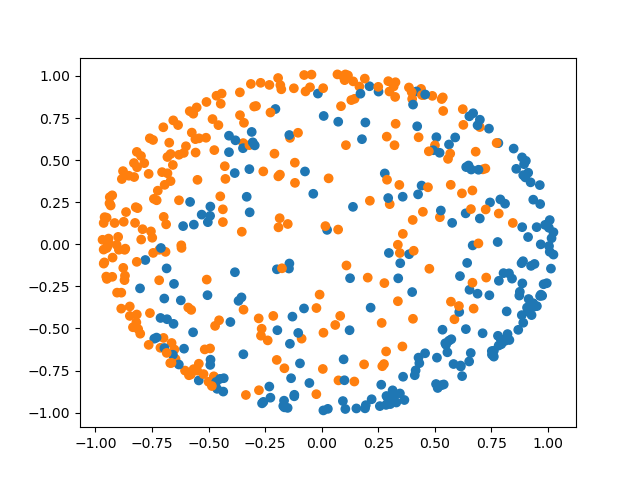
\includegraphics[width=6cm, keepaspectratio]{imports/PCA.png}
        
        \caption{Réduction du dataset Globe}
    \end{figure}
\end{center}

Cette méthode est très performante en termes de temps de calcul et respecte fortement la distance au voisinage de chaque point, cependant elle ne représente pas correctement les classes.
\smallskip
La méthode est implémentée dans la librairie \href{https://scikit-learn.org/stable/modules/generated/sklearn.decomposition.PCA.html}{scikit-learn}.

\subsection{Multidimensional Scaling (MDS)}

Le principe de fonctionnement de cette méthode est de projeter les données dans un sous-espace linéaire\cite{abdi2007-MDS}. L'objectif de cette approche est de conserver de la meilleure façon possible les distances au carré provenant de l’espace des données. 
Pour y parvenir, l'algorithme cherche pour chaque métrique de l'espace des données, une combinaison linéaire optimale. Globalement cette technique a les mêmes défauts que l’ACP quand il s’agit de projeter des données linéairement séparables.
Néanmoins, dû au fait que la cette technique prend une matrice de similarité en entrée, les axes de projection de cette technique ne sont pas directement interprétables\cite{HeulotThese}.

\begin{center}
    \begin{figure}[ht!]
        \centering
        
        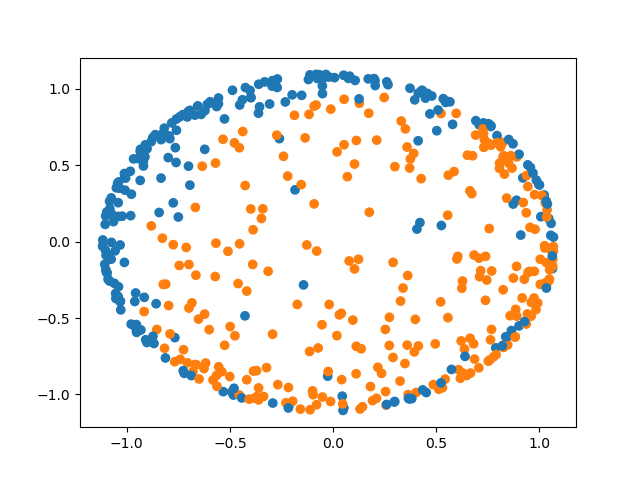
\includegraphics[width=6cm, keepaspectratio]{imports/MDS.png}
        
        \caption{Réduction du dataset Globe}
    \end{figure}
\end{center}

Cette méthode est performante en termes de temps de calcul et de mémoire. Dans le cas du jeu de données \textit{GLOBE} que nous avons utilisé, les classes sont préservées, néanmoins une d'entre elles est projetée à l'extérieur.

La méthode est implémentée dans la librairie \href{https://scikit-learn.org/stable/modules/generated/sklearn.manifold.MDS.html}{scikit-learn}.
\url{{https://scikit-learn.org/stable/modules/generated/sklearn.manifold.MDS.html}}


\subsection{ClassNerv}
 Cette méthode a été présentée lors de la prestigieuse conférence NeurIPS de 2020 \cite{colange_steering_2020}.

 C'est une méthode de projection qui permet de réduire la dimension d'un jeu de données en conservant les classes et leur voisinage. 
 Elle présente les avantages des méthodes supervisées et non supervisés, c'est à dire la combinaison du traitement par classe et par distance au voisinage ce qui permet
 d'eviter de nombreuses erreurs de classification.
 On peut y faire varier les paramètres \[\tau^*=\dfrac{\tau^\in + \tau^{\not\in}}{2}\]  \[\varepsilon=\dfrac{\tau^\in - \tau^{\not\in}}{2}\]  
 $ \tau^* \in [0,1] $ avec 0 pour un minimum de faux voisin et 1 pour un minimum de voisin raté. 
 
 \noindent $\varepsilon \in [0,0.5]$ 0 pour réduire la supervision, et 0.5 pour l'augmenter. 
 
 \noindent
 Par exemple sur le Dataset Globe (deux classes séparées en deux hémisphères, représentation d'origine en 3D), on obtient les résultats suivants :


\begin{center}
    \begin{figure}[ht!]
        \centering
        
        \includegraphics[width=7cm, keepaspectratio]{imports/classNervSphere.png}
        
        \caption{Réduction du dataset Globe}
    \end{figure}
\end{center}

On peut remarquer que l'on obtient un meilleur résultat avec un $\varepsilon$ de 0.25 et un $\tau^*$ de 0.75, c'est-à-dire une supervision moyenne et en privilégiant les faux voisins plutôt que les voisins manqués.
Il est également important de noter que cette méthode est très coûteuse en temps de calcul. 

Le code Python nécessaire pour l'implémentation de cette méthode est accessible : \href{https://zenodo.org/record/4094851#.YaxeoS_pO-w}{ici}.


\subsection{t-SNE}

Cette méthode non linéaire se base sur un algorithme de projection: le SNE \cite{hinton2002-SNE} celui-ci permet de bonnes visualisations, mais a une fonction de coût qui est difficile à optimiser. C’est notamment de ce problème dont le t-SNE s’affranchit en utilisant une fonction coût symétrique  et une t-distribution plutôt qu’une distribution Gaussienne. 
Ces deux changements lui  permettent d’enlever les problèmes d’optimisation du SNE. Cette méthode est donc plus simple et plus rapide à exécuter. De plus, les maps produites seraient même de meilleure qualité\cite{van2008TSNE}.
\smallskip
Avec le t-SNE, il est possible de restituer fidèlement la structure d’un grand jeu de données au niveau local et au niveau global. Cette méthode permet en effet de repérer la présence de clusters à différentes échelles. Il est par ailleurs possible de retrouver les clusters “séparés”, et de faire une approximation du spectral clustering avec un certain paramétrage. \cite{linderman2019Spectral1} \cite{chui2006Spectral2} \cite{von2007SpectralClustering}.
\smallskip

La démarche de cette méthode est la suivante : elle commence par calculer la  probabilité $P$ que deux instances puissent être voisines. Ainsi, la valeur de $P$ sera haute pour des voisins proches et très faible pour des voisins éloignés.\newline
La variance de la distribution Gaussienne est différente à chaque fois, ce qui permet d'enregistrer la densité pour différents voisinages multidimensionnels.
Le calcul va s’effectuer de façon itérative jusqu’à ce que la perplexité (au préalable définie par l’utilisateur) soit atteinte.
\newline Une fois, toutes les probabilités calculées le but est de trouver une distribution de probabilité $Q$ qui représente fidèlement le jeu dans un espace de plus faible dimension. Cette fois-ci, au lieu d’utiliser une distribution Gaussienne, c’est une distribution du t de Student qui est utilisée, avec un degré de liberté de 1. 
\newline Contrairement à $P$, $Q$ n’est pas paramétré avec une variable de densité de voisinage, par conséquent des voisinages avec des densités très différentes dans l’espace original peuvent être transformés en  voisinages de tailles équivalents dans la représentation à plus faible dimension.
La recherche de $Q$ qui représente fidèlement $P$ se fait en optimisant la fonction coût suivant la divergence de Kull-Leibler des deux distributions. Cette étape est effectuée de façon itérative en faisant une descente de gradient pour un nombre d’itérations déterminé par l’utilisateur \cite{van2008TSNE}.

\begin{center}
    \begin{figure}[ht!]
        \centering
        
        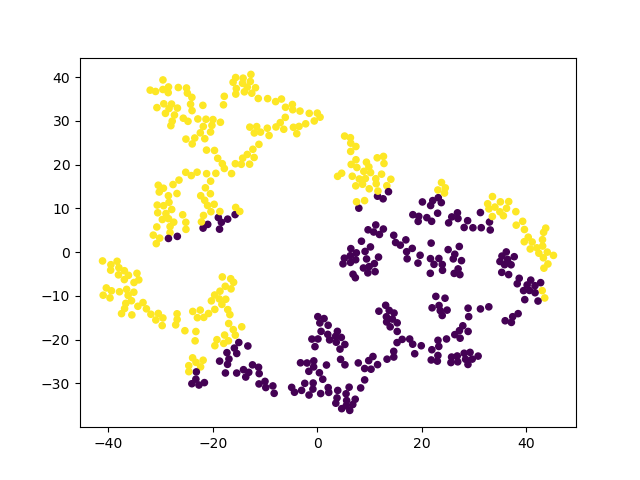
\includegraphics[width=7cm, keepaspectratio]{imports/tsne.png}
        
        \caption{Réduction du dataset Globe}
    \end{figure}
\end{center}

Cette méthode est très performante en temps de calcul, mais cela se fait au détriment des résultats qui sont beaucoup moins précis. 
Les classes sont relativement bien séparées, mais la distance au voisinage n'est absolument pas respectée.

Celle-ci est implémentée dans des projets \href{https://lvdmaaten.github.io/tsne/}{github} par Laurens Van Der Maaten dans une grande diversité de langages (Matlab, Python/Cuda, R, ...). 

\subsection{Autres méthodes de projection non linéaires}
La liste des méthodes de projections non linéaires ne se limite évidemment pas à celles citées.
Nous pouvons également retrouver le Sammon mapping\cite{sammon1969nonlinear}, le \textit{curvilinear components analysis}(CCA)\cite{demartines1997curvilinearCCA}, le \textit{Maximum Variance Unfolding}(MVU)\cite{weinberger2006MVU1} \cite{song2007MVU2}, 
ou le \textit{Laplacian Eigenmaps}\cite{saul2000introduction}. 
Ces techniques sont performantes, mais peinent à être efficaces quand il s’agit de visualiser des jeux de données avec beaucoup de dimensions. Il nous était également compliqué de restituer correctement les structures locales et globales dans une seule projection\cite{belkin2002semi} \cite{van2008TSNE}.
C’est en partie pour ces raisons et le manque d'implémentation disponibles qu'elles n’ont pas été retenues pour notre projet.
\smallskip


\subsection{Conclusion de la partie}
Comme nous avons pu le voir, il existe de nombreux algorithmes de projections qui se basent tous sur différentes hypothèses mathématiques, différents critères et différents paramétrages. Ainsi, avec un même jeu de données, il est possible d'obtenir plusieurs projections différentes en fonction des algorithmes choisis(le nuage de points ne sera pas le même) . 
Le choix du type d’algorithme de projection à utiliser dépend de la nature des données que l’on veut étudier, du type de résultat que l’on souhaite observer et de nombreuses caractéristiques propres aux données qui peuvent être très complexes à appréhender sans de bonnes connaissances en projection de données.

Par exemple, nous avons vu pour L’ACP et Isomap, qu'elles ne sont pas stables face aux variations des données. La raison est que l'ajout ou la suppression de quelques instances peut modifier de manière significative les vecteurs et les valeurs propres, affectant ainsi considérablement la cartographie. Même de petites perturbations dans les données peuvent avoir un impact conséquent sur la cartographie finale en raison de l'inversion des vecteurs propres. Ce qui entraîne des configurations très différentes avant et après la perturbation \cite{nonato2018multidimensional}.
Le t-SNE quant à lui est basé sur des procédures d'optimisation dont la solution optimale dépend des conditions initiales. En général, des initialisations différentes conduisent à des solutions différentes. La stabilité n'est pas garantie même en fixant la condition initiale, de sorte qu'une modification du nombre d'éléments peut conduire à des agencements sensiblement différents \cite{garcia2013stability}.
Quant au MDS, c'est une technique qui repose sur des points de repère ou de contrôle et qui a tendance à être stable tant que les points de contrôle et de repère restent fixes. Comme la position de chaque instance ne dépend que des points de contrôle (points de repère), si ces points ne changent pas, le mappage ne change pas non plus \cite{garcia2013stability}.


Nous pouvons donc affirmer qu'aucune méthode n’est parfaite : peu importe la réduction de dimension appliquée une perte de données est inévitable ce qui cause forcément l’apparition d’artefacts. Ce qui soulève la question suivante : Comment s’assurer de la qualité d’une projection ? 
Pour appréhender cela, nous passerons en revue plusieurs critères et méthodes d'évaluation de la qualité d'une projection dans le chapitre suivant.



